\documentclass{standalone}
\usepackage[T1]{fontenc}
\usepackage[utf8]{inputenc}          % needed for French accents
\usepackage{pgfplotstable}
\usepackage{pgfplots}
\pgfplotsset{compat=1.18}
\usepackage{siunitx}                 % optional, nicer y‑axis numbers
\usepackage{booktabs}                % pretty tables for the optional preview

% -------------------------------------------------
% Helper that removes the internal \pgfpl@@ wrapper
% -------------------------------------------------

\begin{document}
% This file was created with matplot2tikz v0.4.0.
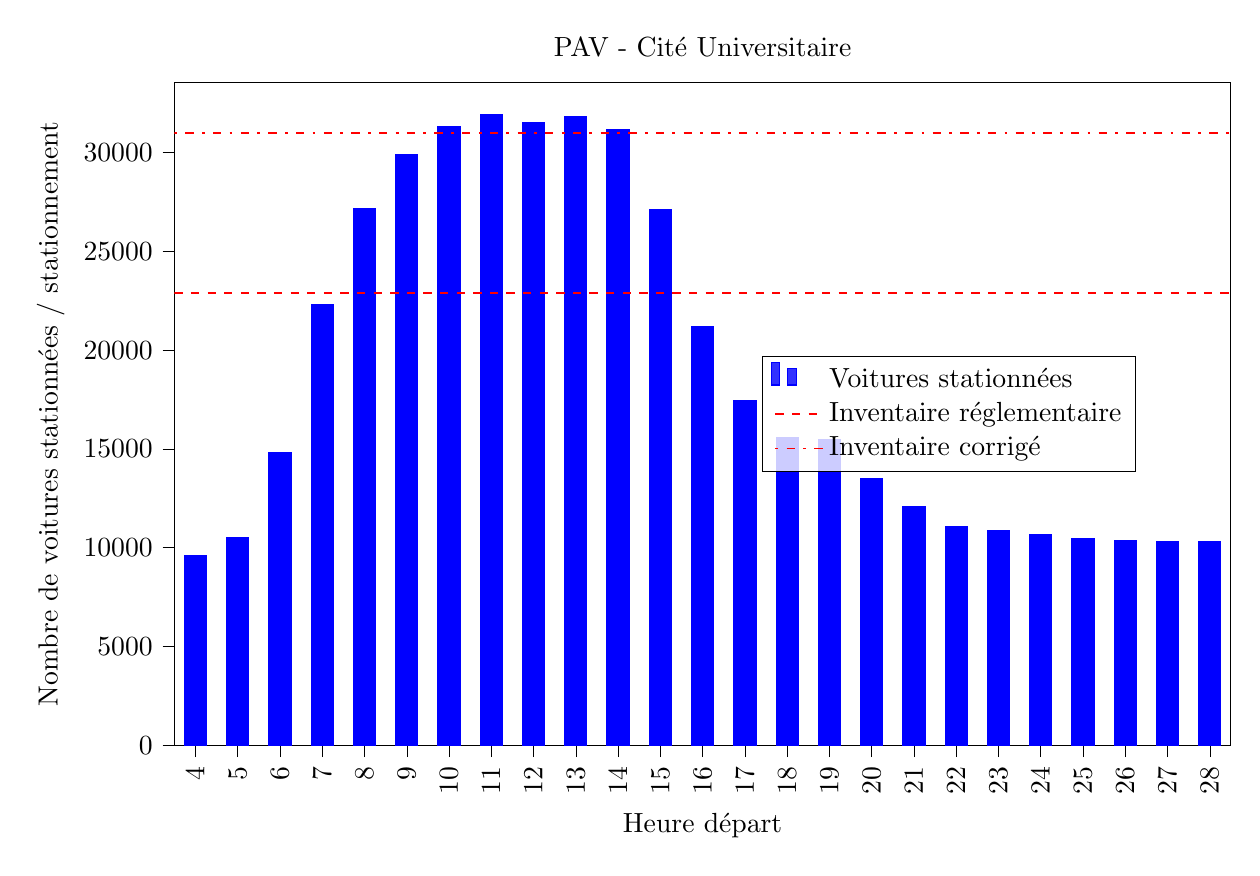
\begin{tikzpicture}

\begin{axis}[
height=10cm,
legend cell align={left},
legend style={
  fill opacity=0.8,
  draw opacity=1,
  text opacity=1,
  at={(0.91,0.5)},
  anchor=east,
},
minor xtick={},
minor ytick={},
tick align=outside,
tick pos=left,
title={PAV - Cité Universitaire},
width=15cm,
xlabel={Heure départ},
xmin=3.5, xmax=28.5,
xtick style={color=black},
xtick={0,1,2,3,4,5,6,7,8,9,10,11,12,13,14,15,16,17,18,19,20,21,22,23,24,25,26,27,28},
xticklabel style={rotate=90.0},
ylabel={Nombre de voitures stationnées / stationnement},
ymin=0, ymax=33543.3,
ytick style={color=black},
ytick={0,5000,10000,15000,20000,25000,30000,35000},
yticklabels={
  \(\displaystyle {0}\),
  \(\displaystyle {5000}\),
  \(\displaystyle {10000}\),
  \(\displaystyle {15000}\),
  \(\displaystyle {20000}\),
  \(\displaystyle {25000}\),
  \(\displaystyle {30000}\),
  \(\displaystyle {35000}\)
},
scaled ticks=false
]

\addplot[ybar,draw=blue,fill=blue,legend image post style={/pgfplots/ybar legend},
  bar width=8pt]
        coordinates{
            (4, 9608)
            (5, 10509)
            (6, 14792)
            (7, 22315)
            (8, 27168)
            (9, 29920)
            (10,31334)
            (11,31946)
            (12,31497)
            (13,31825)
            (14,31150)
            (15,27124)
            (16,21186)
            (17,17449)
            (18,15569)
            (19,15459)
            (20,13518)
            (21,12062)
            (22,11076)
            (23,10849)
            (24,10675)
            (25,10462)
            (26,10376)
            (27,10320)
            (28,10320)
            };
\addlegendentry{Voitures stationnées}
\addplot [semithick, red, dashed]
table {%
3.5 22883
28.5 22883
};
\addlegendentry{Inventaire réglementaire}
\addplot [semithick, red, dash pattern=on 1pt off 3pt on 3pt off 3pt]
table {%
3.5 30976
28.5 30976
};
\addlegendentry{Inventaire corrigé}
\end{axis}

\end{tikzpicture}

\end{document}